
\documentclass{report}
\usepackage[utf8x]{inputenc}
\usepackage[english]{babel}
\usepackage{url}
\usepackage{graphicx}
\usepackage{imakeidx} % for how to use the index see https://www.sharelatex.com/learn/Indices
\usepackage{hyperref}
\usepackage[margin=0.6in]{geometry}
\usepackage{afterpage}

\newcommand\blankpage{%
    \null
    \thispagestyle{empty}%
    \addtocounter{page}{-1}%
    \newpage}


\title{Trash Magic Action Coloring Book}
\author{Trash Robot}

\begin{document}

%\thispagestyle{empty}
%\mbox{}
\maketitle

\section{Trash Magic}

We will build a world of both comfort and adventure from the waste streams of the old world.  We will use the trash we find everywhere to build all the things of a good life right where we are.  We will power this technology only with the sun, wind and water.  We will abolish all mining, oil, and gas by 2050.

Magic is the replication of the desire to replicate something.  If someone builds something out of trash which someone else wants to copy, and which will lead to still more people copying it, that's trash magic.  

Full trash magic is when we have trash magic technologies which taken together provide for all the things we need for a very good life.

To build this we will create Trash Factories.  A Trash Factory is a manufacturing hub which consumes waste from the local environment and converts it into products to directly provide to people in the local community.  Trash factories use only what is in their immediate physical environment for motive power.  This primarily means human power, direct solar heat, flowing water from rivers or tides, and wind.  It can be electrical, but can also be direct mechanical, as was common before universal electrification.  

Trash factories aim to close the loop of machine replication. This means we want the factories to have metal shops with all the basic tools of machine fabrication: milling machines, lathes, drill press, plastics welding and molding, welding and soldering, sheet metal working, etc.  With all these basic mechanical fabrication tools, we can in turn make more of these tools in that shop, using waste streams of metal found in our community.  

In order for trash factories to propagate, we will need very simple and clear instructions built into self-replicating media which describe how to replicate each part.  We also need a training corps who will go and recruit people to build trash factories and teach them how to do it.  Instructions should themselves be replicated as many times as possible, with new people recording their own videos on video sharing platforms, so that our media keeps improving.  

This book is a magic book, which will be self-described in the next chapter.  The fact that this book replicates means that as we add little bits and pieces of full trash magic, it will replicate as the book is copied and edited out in the wild.  

In addition to the machine shop, trash factories will be centered around textile fabrication again from waste.  We will use the machine shop to build machines for drawing plastic waste out into filaments, spinning it into thread, weaving it into cloth, and stitching it into clothes.  We will build machines for blending different materials into custom fibers for our own textiles which are based on what we can get our hands on. 

The textile part of the factory is our main initial product.  We need to have fiber arts experts and fashion designers involved at all stages of putting this together, so that we can build both practical and awesome looking stuff, custom designed for all body types.  Because we are supplying only our physically local community, all clothes are custom by default.  Our first priority in all clothing production is to provide survival gear to the most vulnerable people in our immediate physical community. From there we aim to create new fashions which blend practicality and comfort with post apocalyptic trash witch rainbowcore aesthetic.

For motive power we need the machine shop to also immediately be constructed around a standardized solar heat engine of some kind which can drive about 500-1000 watts, as well as a standard equivalent with wind and water.  This needs to have again a standardized system of shafts, pulleys and belts for power transfer to various machines as we add them as well as to electrical generators.  

For energy storage we need a standard water turbine and pump design which can be used to pump water uphill then run it downhill to get the energy back out.  We also need a battery solution we can make with safe waste streams.  We do not care about getting insanely high energy density or low weight.  Many ideas should be explored but we think the aluminum carbon cycle is perhaps the best choice, as we can get aluminum from beverage containers and carbon from locally produced charcoal.  Also, we need to create a reliable process for combining spent lithium ion cells and bringing them back to life.  

All the parts of the trash factory are intended to be things which can be either a purely trash-factory built thing or a off the shelf thing we can buy as we get started.  We cannot expect to build a fully closed loop trash factory immediately.  We instead aim to get something which creates value as fast as possible. 

Trash Camps are mutual aid centers in public spaces where we provide direct help to people in those spaces.  These camps are the retail distribution for the products we make in the trash factories.  Our aim with trash camps is to as quickly as possible have them provide some value to people in their infrastructure on site as well as a distribution point for a flow of free things to the most disenfranchised.

Trash academies are centers of learning for the community to learn about technology which is relevant to the trash magic system.  This includes both vocational training directly in how to operate the parts of the trash factory and more general education in all of the things we hope young people to know in the trash magic future.  What makes a trash academy different from an existing school is the lack of formal organizational structure but the much more clear intention of all the work done.  We might do this work in a public library, a university, a public park, on a huge raft made of trash, in a government lab or under a bridge. But wherever we do it we will do everything with the constant vision in mind that all our labors are in the direction of full trash magic.

Initially our trash academy education will have a few specific topics which we can immediately share in trash camps as a form of mutual aid because it can help people to survive right now.  This includes teaching people to make their own web pages, teaching them to make their own web-based applications, teaching people to build their own wireless networks, to build their own off-grid power.  We also have an open source Arduino development class.  If we build basic educational tools into the trash camps, and we have highly qualified technical instructors, we can mix teaching the most under-resourced students with helping the more privileged students whose families can then help us with resources.  

The trash academies will ultimately also serve as centers for research and development as we grow, which will be called Trash Labs.  However, again, our initial focus is to provide value and to replicate first.  So initially we focus on the maximum educational benefit to the most disenfranchised, which is primarily technology education for getting direct control of their own social media platforms using the magic books(see next chapter).  Focusing on technology education allows us to 

\begin{figure}
	\centering
	
\includegraphics[width=5in]{imageserver/uploadimages/image3.png}
	\caption{Magical symbology. What are our symbols? What represents who we are and what that means?  What are our most organic symbols, which most freely replicate from person to person?}
\end{figure}


\begin{figure}
	\centering
	
\includegraphics[width=5in]{imageserver/uploadimages/image12.png}
	\caption{Magic.  Replication in all directions.}
\end{figure}

\begin{figure}
	\centering
	
\includegraphics[width=5in]{imageserver/uploadimages/image13.png}
	\caption{Magic trash.}
\end{figure}

\begin{figure}
	\centering
	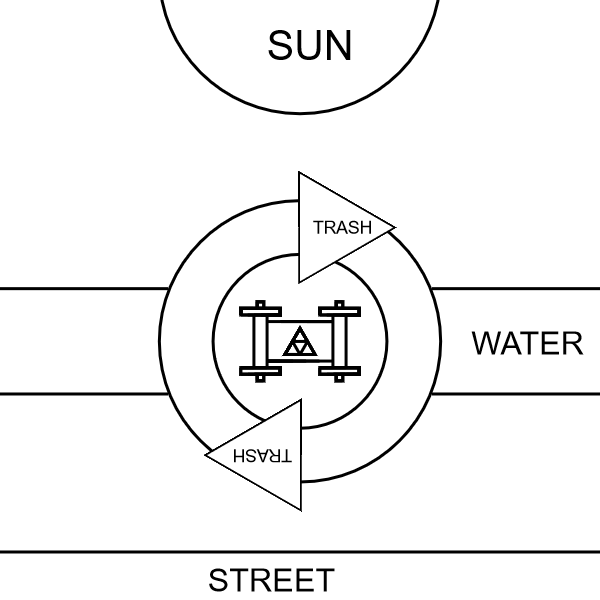
\includegraphics[width=5in]{imageserver/uploadimages/image14.png}
	\caption{Trash magic map.}
\end{figure}

\begin{figure}
	\centering
	
\includegraphics[width=5in]{imageserver/uploadimages/image15.png}
	\caption{Trash magic graph.}
\end{figure}

\begin{figure}
	\centering
	
\includegraphics[width=5in]{imageserver/uploadimages/image3.png}
	\caption{Trash Factory. List the things available from the trash factory here.  What are the products, and how can people get them?}
\end{figure}

\begin{figure}
	\centering
	
\includegraphics[width=5in]{imageserver/uploadimages/image3.png}
	\caption{Trash Feed. Where are we getting trash from? What trash? From whom?  List trash sources, people, places, things.}
\end{figure}

\begin{figure}
	\centering
	
\includegraphics[width=5in]{imageserver/uploadimages/image3.png}
	\caption{Community resources. Our whole purpose is to provide aid to the community. List community resources here.  Who needs what, and how can they get it? Post contact information of both those in need and those willing to help.}
\end{figure}


\begin{figure}
	\centering
	
\includegraphics[width=5in]{imageserver/uploadimages/image3.png}
	\caption{Trash Camp. Where are we hanging out?  Details of a spot go here, this can be maker spaces, schools, community centers, parks, or just spaces we can exist.  Draw maps, list places, add links.}
\end{figure}


\begin{figure}
	\centering
	
\includegraphics[width=5in]{imageserver/uploadimages/image3.png}
	\caption{Trash Academy: Teaching. Who is teaching what, and where?  List of what's offered and who teaches it and where they are, contact info of teachers, links to resources to learn.}
\end{figure}

\begin{figure}
	\centering
	
\includegraphics[width=5in]{imageserver/uploadimages/image3.png}
	\caption{Trash Labs: Research and Development.  Research path.  What do we need to figure out how to build next? What are we working on now?}
\end{figure}

\section{Magic Book}

The magic book is a book which you co-create with other readers and writers.  It can replicate freely along the Geometron network, as described in the Book of Geometron.  This is not a specific book so much as a collection of methods of creating self-replicating books.  

The formats of the books are hand drawn and hand bound zines, bound 6x9 hard copy printed by print on demand Lulu press, printed letter size paper in three ring binders, and a web-based format which is how text is edited.  The web books have code in them which allows them to replicate freely from one Geometron server to another.  

As a keeper of any given version you will have received it from someone who can show you how to pass it along.  You can just pass along a book from one person to another and track it in the Street Network chapter. 

The electronic magic book can be part of an event, including a virtual one, where people message additions to a document to a human operator who edits the document in real time and shares it over a web server with everyone, who can then replicate it again, edit it again and so on.  This can be done on a Raspberry Pi, the cheap open source computer platform used for everything in the Geometron network. 

The Magic book can be used for many things. It can be used to co-create a story.  It can be used to create a shared book documenting a local community. It can be fiction or non-fiction.  It can be many hundreds or even thousands of pages, or just a single page with a short list of links.  It can be entirely images or just text.  What makes it magic is that it can always be replicated and edited by each new person we share it with.  As with trash magic, this fits our working definition of magic: the book replicates the desire to replicate the book.  

The Magic Book can also have oral formats, either from memory in person, over live stream, on a video sharing platform, or on an audio podcast.  Or it can be entirely performance art as we carry out the actions which are encoded in the book, just building and sharing geometry. 

\begin{figure}
	\centering
	
\includegraphics[width=5in]{imageserver/uploadimages/image16.png}
	\caption{Scroll.}
\end{figure}

\begin{figure}
	\centering
	
\includegraphics[width=5in]{imageserver/uploadimages/image17.png}
	\caption{Infinite scrolls.}
\end{figure}


\begin{figure}
	\centering
	
\includegraphics[width=5in]{imageserver/uploadimages/image3.png}
	\caption{Prompt of prompts. Keep track of useful prompts to add.  These are blank pages with a caption which describes what goes in them, or digital scrolls with the prompt at the top.}
\end{figure}


\begin{figure}
	\centering
	
\includegraphics[width=5in]{imageserver/uploadimages/image3.png}
	\caption{This book.  Notes on this book, self-documenting. Where it went, where it goes.}
\end{figure}


\section{Street Network}

The consumer society we live in today relies on a vast and
well-organized collection of networks to function. There are the
networks which channel freight from one place to another, like trains,
trucks and boats. There are the human transport networks like planes,
personal cars and buses. There are the invisible networks of power based
on who when to school with whom, family connections, or business
connections. And of course there is the global information network
centered on the Internet which connects everyone together by
information.

What we seek to build is the means of replication of trash-based
technology in order to propagate our new civilization built entirely
from trash. This new system will be much more localized than the
existing one. Rather than needing a constant high rate of movement of
very large quantities of physical goods, we plan to build systems which
will ultimately use material directly available in our physical
environment rather than from far away. Even in places with limited
agricultural capacity, I believe that with the superior technology which
we can build using a more organic system that we can build dense food
production and water purification everywhere once we put our minds to
it, making almost all large scale movement of goods un-needed. We will
still move goods and people, but more by choice than necessity for
personal reasons. When globalization does not force everyplace to be
identical, travel can become an adventure again!

Part of the ideology of the existing Internet-based culture is that
place no longer matters. People appear on a teleconference or send an
email and no one cares where they are. People arrive for a meeting in a
business hotel or conference center and it is identical to every other
place in the world. The ideological basis of the Geometron Street
Network is that place \emph{does} matter and \emph{should}matter. We
reject the idea of ``nowhere''. Everyone is somewhere. Whether you are
in a rural area, a suburb, a big city or a highway rest stop you are
always \emph{somewhere}. Furthermore, that place you are has its own
local geographical logic. It has its own crossroads, its own nodes of
power and connection, whether it is the local pub or coffee shop or the
exit of a subway station. All these little places on the scale of one
human body have real meaning for the people who inhabit that space.

We want an information network based around physical replication of
technology from trash. To stimulate the replication of the Network, we
need it to create value for people who use it and operate it. This value
can be of many kinds: it can directly provide physical goods people
need, it can facilitate business in the monetary economy, it can provide
mutual aid to a community, it can create local social connections, can
build network power for users, and any of these values can be traded for
materials and space needed to continue to expand the network.

The Street Network consists of the people going out and spreading all
this, the web servers we use to do it, and globally visible web pages
which serve as links to connect users to us and our network.

We buy domain names which are linked to a place but not property. We
avoid .com and focus on .org, .net or .xyz domains. We avoid specific
addresses or names of companies. We choose names that describe shared
resources which are public enough that no one is in the position to
claim ownership of the name. This can be the name of a neighborhood or
street, a body of water, a park, or a mobile shared resource like a
mutual aid bus used by people who already do not use property. In the
physical location described by the domain we create and share physical
media which points to the domain. In its simplest form this can just be
a hand written cardboard sign. However, we can also use Geometron to
make various self-replicating physical media which transmit the domain,
such as laser cut spray stencils and the self-replicating clay tokens
described later in this work. We also can fly a black flag of the place
with cut out colored felt sewn on a black square of cloth, which is
described in the Scrolls distributed with the system.

Each domain is hosted on some commercial server for the time being, from
providers such as Dreamhost or Bluehost. Free web hosting can also be
used at 000webhost.com and is recommended if you have no money. The
Geometron software can then be installed on each of these servers
according to the instructions in the next section(and repeated on each
Geoemtron instance in the Scrolls), making it just another identical
instance of the software to what exists on all the local Raspberry Pi
based servers. The primary purpose of these globally visible domains is
to point back to the local server. In its simplest form this is just a
description of when and where you might find the server. Photographs of
the network Operator and their gear can validate the system to passerby.
The Map format described in a later chapter can also be used to
precisely identify physical places where infrastructure can be found.

The deceptively simple structure described above is the Street Network.
We are adding digital media technology to the oldest network in the
world: the physical paths of movement. We will use this to follow all
those paths, from superhighways to ancient footpaths to natural harbors,
just as other ideas have traveled throughout human history. If we find
the most powerful nodes of geography we can build a network of
staggering power with a relatively small number of people initially.

\hypertarget{users}{%
\subsection{Users}\label{users}}

The uses of this network are very different for different people, just
as is the case for the existing global networks like the Internet. In
this section I will discuss some of the different user groups and how
our network can provide value for them.

\textbf{Operators.} We are the start of this. Get a Raspeberry Pi and
install the system. Get a domain, install the system and point to your
server. Go forth and share! Ultimately those of us who build and share
this system will form a very powerful network of mendicants. The
mendicant tradition has appeared many times in many places in history. A
mendicant is someone who is totally devoted to their faith(they are
generally religious orders) who renounces wealth and travels with no
possessions asking passerby for donations to support them. This has
traditionally created contradictions, as these orders have a way of
gaining power and becoming anything but poor as they scale up. As our
consumer society has destroyed itself it has driven more and more people
into this way of living against their will. If our network provides vast
amounts of value to people we will find that the most marginalized
people of today when leveraging the power of this new network can barter
for not just survival but to thrive in a new civilization without money,
mining or property.

We follow the laws of Geoemtron listed in the previous chapter as a
guide for building this new world. We teach everyone we meet how this
whole system works, and recruit new people as Operators. Note that the
idea of a mendicant order has strong religious overtones, but that this
is a completely non-denominational order based on the universal language
of geometry. Geometry has a central place in all existing cosmologies,
both ones considered religious and ones considered secular. The work
here presents a way of interacting with the world based on geometry. In
some ways this whole project can be thought of as the start of a free
school for teaching a new kind of geometry. This is a distant descendant
then of the geometry schools of the ancient world. We teach people the
whole system; mathematical philosophy, robotics, code, all kinds of
industrial fabrication, crafts, fashion, whatever we build we teach and
share freely.

Do not misinterpret this idea of the mendicant as a vow of poverty. We
will be more wealthy than anyone currently living in the consumer
society once we scale this Network. We are building a new world in which
no one is poor. By starting from a baseline of people who have nothing
but building better technology than what is presently available in
consumer civilization we start by making sure those who have the least
have everything: free clean water, free good food, free high technology
medicine, free transport, free shelter, free network technology, free
air conditioning and heat etc. If those who have the least have better
stuff than the richest people in today's world the world of today will
dissolve and be naturally replaced by this new order built from the
waste of the old.

\textbf{Traveling kids, hobos, panhandlers, people asking for money or
selling things on the street corner.} A physically local free bulletin
board shared by passerby in a high traffic area can allow people asking
for money who are currently ignored by passerby as just another
anonymous face and cardboard sign a chance to really tell their stories
and to share all that they have to share. When people share their
stories they can become part of the emergent physical community of
passerby in a location where the network node is located. When people
view others as part of their community they not only are more willing to
help, they can have open communication about the best way to help,
expanding from just spare change to more comprehensive mutual aid.
Because we clone content from the local terminal to web pages on
globally visible domains linked to a physical place, which are
advertised everywhere in that place, marginalized people whose only
ability to get online is the public library can use the computers there
to get the information they need to better survive, and ultimately to
thrive and build new communities where they already are. The way a local
network can help people is twofold. First, it is direct, by asking for
money and other mutual aid. But by being physically on location all the
time, already with physical media(cardboard signs), people in a given
place can aid the network, creating value for the other people in the
community who are more resourced, who then no longer view monetary
support as ``donation'', but rather as an expense which supports their
other business activities.

In order to see the power of this second means of network support of
marginalized people on the street, we have to look more closely at the
network nodes we are building. One of the major types of node is in a
business district of a city where there are both homeless people asking
for money, on the street all day with physical media, and power brokers
who make their living entirely from connections. These people include
venture capitalists, entrepreneurs, lobbyists, consultants, and the rest
of what might be called the ``deal-making class''. An example of this
confluence is some of the parks along K-Street in Washington DC. K
Street and adjacent streets is home to a huge homeless population as
well as power brokers whose livelihood depends entirely on connections.
If a physical network were built which facilitated direct communication
between people along K Street, the people who spend the most time
physically on the street can be brokers of information on a network
which can be worth a lot to the people who trade in information.
Physically local information networks can leverage the power of physical
places with very powerful people walking past all the time who normally
never communicate. Connecting these people up can be dangerous. But if
we provide them with value, it can be worth both a lot of money to them
and also potentially something they can barter for giving us space to
live and work nearby. If you facilitate a 10 million dollar deal and the
customer knows you can do it again, the least they can do is give you a
100 dollar gift card to the nicest restaurant in the block. There is no
real upper limit on what an enterprising Network Operator could in
theory make if they learned to really channel information efficiently in
the nodes of global power. And of course we must remember that when
dealing with power brokers their currency is not money. When the people
who currently have the most power in society find themselves dependent
on free open networks, those networks themselves will gain power which
penetrates that of the existing power structures, potentially creating
an existential threat to them. We must take note of this.

The elements of traveler culture which overlap with ``van life'' are
also key to increasing the network effects of the Street Network. This
also links to trucker networks. People who live their lives on the road
can use this network infrastructure to set up complex networks and
markets in highway rest stops, Walmart parking lots etc. using either
wifi networks in these places or their own hotspots from their phones.
These networks can be of utility to passerby of all kinds, from tourists
to truckers to the workers who keep the places running. Just as existing
global social media networks provide value they can charge money for, a
physically local network can provide value which people will pay for. An
example use case here is a Street Network Operator agreeing to maintain
a backup of and keep posting an advertisement for something a local
entrepreneur is trying to sell to truckers. In exchange for that, they
can get directly compensated in gas, right there in the rest stop,
without money changing hands.

\textbf{Food not bombs, street outreach, harm reduction people, mutual
aid workers.} See above. The people who are working to help the most
marginalized members of any given community can better reach that
community if there is a physically local media platform where people can
share information about resources. Documents can be posted which explain
how to get access to resources, when and where resources will be
available, etc. Because the whole system self-replicates, as with Food
Not Bombs, anything which is successful in any given place can be
immediately cloned to other nodes on the network. Food Not Bombs already
has a global network of free and open nodes with no property but a very
recognizable brand identity and set of behaviors and actions. FNB nodes
are generally already linked by networks both online and via people who
travel from one punk house or FNB house to the next. The whole anarchist
network of community houses, FNB's, anarchist infoshops and bookstores,
really really free markets, free boxes, etc. can form a basis for a
truly free information network carried from house to house and city to
city, running on house wifi networks.

\textbf{Business owners in a shopping center.} Every business owner has
neighbors who are also business owners. You already have an informal
network. But installing free digital media infrastructure can provide
huge value by allowing more mutual aid between neighbors of all kinds,
both owners and customers. Tech giants ignore you. They demand monetary
tribute in order to even have your business listed, and then still
refuse to give you an equal footing to the corporate giants which
dominate their platforms. By controlling a local platform in \emph{your}
shopping center, you can provide value to customers with articles they
write and share with one another which brings them in(just as
advertising-supported media has interesting content to get people to
look at ads). And then this medium can have much more than just the ads
you would get from a Big Tech platform. You can post really detailed
information about everything you do with no restrictions on length, and
share across the shopping center. If you own a karate school next to a
dentist, the bored people in the waiting room can read about the history
of karate right next to a detailed schedule of your class offerings. And
when parents wait for their kids to get out of karate class they can be
reading about clean gums in an article written by the dentist. Big Tech
doesn't care about you. If you build your own network, you can center it
right where it belongs: on the people actually using it, rather than a
few oligarchs in San Francisco.

\textbf{Coffee shop owners.} Building a network in a coffee shop on the
wifi network which requires purchase to use and which has a time limit
can create a huge amount of added business for any local business owner.
It also builds community. So coffee shop owners who find themselves with
a full shop of laptop drones with headphones on who work for hours, or
get kicked out and do the same thing somewhere else can instead find
themselves the brokers in a very powerful information network. Much of
the commerce of the world is now code written in coffee shops on
laptops. Creating physically local networks around these already
existing groups can create huge power for the users which then benefits
the people who set up the infrastructure(again, just like existing
centralized social media platforms.)

\textbf{Web developers.} We need web developers(people who can write
HTML and JavaScript code) to be constantly writing more and better
software in order to make Geometron a success. Developers who work all
day in coffee shops or any other shared space like a co-working space or
pub can have a social network based on both co-developing applications
useful to all and sharing other resources. Developers will use the
resource of the Street Network terminal/server on the local network in
the same basic way as others: they can share their resumes, links to
pages of personal projects. Developers are key to the whole system. We
must recruit developers with this book who will rewrite all the code and
also the book, replicating the whole system. The faster our network can
get developers into the swarm, the faster the code itself will improve.
Developers are key!! Developers create servers to share into the
network. I now ask the reader to look up ``steve balmer developers'' on
YouTube.

\textbf{Power brokers.} Venture capitalists, financiers, entrepreneurs,
deal-makers of all kinds, lobbyists, politicians. Your network is your
power. Geography matters. Build a network in the lobby. Post things on
street nodes, build your network, build your power, build your literal
street cred. Deal flow. Deal flow the likes of which you have never
seen. Leverage the power of the physical street!

\textbf{Crafters, makers, jewelers, artists.} An alternative to Etsy,
street vending, or being in a shop. Post your stuff to the local
networks. This is much more free and long form than existing platforms,
you can post images, descriptions, contact info, times and places when
you'll be in a place. This can be way easier than other sales channels
for arts and crafts. You can say when and where you'll be at a place,
post a link for contact, and then show up in the network node like a
coffee shop to make the physical exchange. In many cases, because the
network is physical and local, there will be barter opportunities as
well as direct sales. A barter economy can develop where people donate
materials you use for your crafts as part of how they pay for the
finished product. Removing shipping or transport costs by dealing
directly in a physical location removes friction from the market,
amplifying dramatically the power of the market, especially for crafts
which involve physically bulky objects. For instance, people can bring
in motors and properly prepared plastic sheets and cardboard, as well as
rolls and rolls of duct tape, and we can exchange finished products
built from these materials and tools, as well as free food, drinks, and
supplies, creating a market economy without money as well as without
formal business structures(making it easier for marginalized people to
participate).

\textbf{Any labor pool of gig economy workers focused on a specific
geographic location.} One of the most obvious of these is the drivers
who presently drive for the major rideshare apps who all congregate at
the airport to pick passengers up in the same exact place, and yet all
of it is currently coordinated via the apps(unless you do the cab line).
The rideshares apps have proven that cities will ignore illegal cabs if
they're done at scale. It would be straightforward for a small team of
Network Operators to run a server which replicates to a page which is
advertised around, something like a domain of yourairportnamerides.xyz,
which tells users how to log onto the wifi network created by an
Operator's hotspot near the pickup zone and with a link on the page to
the local network address of the server. All all this IT is doing is
directing customers to a dispatcher who manages the drivers over a
simple app shared by the collective. The whole network is run by a team
of about 2-4 people. One person might be a developer, who creates the
app to manage all the drivers and post messages from dispatch. Another
person is all marketing, putting up the relevant information in the
right places to get seen by travelers but not stopped by the rideshare
apps, airport authorities, or the cab companies. Riders will never have
their destination information on the public network, nor will drivers
put personal information, but they can work on an open trust model where
they are known by dispatch, who has code names for them, and operates a
queue app which simply adds drivers as the arrive near the Airport and
pushes the most senior driver to the top of the stack, which is passed
along to a rider. Another Operator might be the one who runs the trust
network for the drivers, verifying everyone and organizing meetings for
the whole cooperative. This can be used to unionize existing workforces
quickly as well, building ad hoc networks which are very hard to
suppress visible to everyone on their mobile devices on a local wifi
network.

The same model holds for places where workers congregate looking for
short term construction work. Those locations can have a server where an
Operator runs a labor marketplace where a much larger and deeper labor
pool can now advertise, but without all having to be in the physical
location. This means a crowd of a dozen workers looking for work can be
replaced by an Operator with a sign pointing to the domain where the
copy of the market is hosted. Workers who come by can leave an ad on the
local Raspberry Pi Geometron server, and anyone coming by looking for
construction labor can just scroll through a now much deeper collection
of ads and call whoever they need to hire. A market place like this can
suddenly go from a dozen general laborers to a construction labor market
which includes specialists like plumbers and electricians as well as
much larger general contractors just looking to save on marketing costs.
A person holding a cardboard sign on a street corner by a giant box home
improvement store can now potentially be the broker of an information
network on which millions of dollars of commerce flow.

\hypertarget{trash-robot}{%
\subsubsection{Trash Robot}\label{trash-robot}}

The Trash Robot is a self-replicating set of things described later in
this work. It consists of an open brand combined with a way to create
self-replicating symbols which represent in principle anything one can
express with language. We use the Geometron system and the Street
Network as a vehicle to distribute Trash Robot.

Trash Robot icon printers form the basis of a symbolic economy. This
means that we construct self-replicating physical media which can have
symbols representing anything, and we use these symbols to communicate
with each other about how to replicate things. In a numerical economy we
exchange money for goods or services based on a numerical evaluation of
the ``value'' of those goods or services. In Trash Robot we use the
Geometron language to make constructions of pure geometry which can be
used to organize our thoughts and discussions as we share with one
another self-replicating technology of all kinds.

Trash robot consists of a collection of methods for building the robots
and operating existing machines to make all these icons symbols, as well
as the open brand of the fashion and accessories and arts and crafts
which symbolize the system. This brand consists of googly eyes,
rainbows, black cotton flannel, cut felt and rainbow duct tape over
cardboard and bamboo. By being a very recognizable brand identity which
is generic enough to be impossible to copyright, we make a vehicle for
technology which is not property to freely replicate.


 \begin{figure}
	\centering
	
\includegraphics[width=5in]{imageserver/uploadimages/image3.png}
	\caption[streetmaps]
	{Draw maps for the region's streets, one for the major highway corridor, one for local major streets and one for the specific neighborhood.}
\end{figure}

 \begin{figure}
	\centering
	
\includegraphics[width=5in]{imageserver/uploadimages/image3.png}
	\caption[watermaps]
	{Draw maps for the region's water, one for the ocean and major shorelines of your watershed, one for major rivers or lakes and one for immediate drainage.}
\end{figure}

 \begin{figure}
	\centering
	
\includegraphics[width=5in]{imageserver/uploadimages/image3.png}
	\caption[people]
	{The path of this book: people.  Put your name, logo, symbols, signs, links, social media, contact as you see fit, then pass the book along to the next person.}
\end{figure}

 \begin{figure}
	\centering
	
\includegraphics[width=5in]{imageserver/uploadimages/image3.png}
	\caption[places]
	{Keep a record of the travels of this book.}
\end{figure}


\section{Trash Robot}

Trash robot is rainbow and googley eyes.   Trash robot is geometric constructions from cardboard with rainbow duct tape.   Trash robot is felt cutouts on black cotton flannel or sweat pants material.  Trash robot is post apocalyptic trash goblin energy.   Trash robot is chaos.  Trash robot is anarchist science. It's dirty kids in a school bus camper. It's a party by a dumpster.  It's running around in some steam tunnels.  It's weird art dropped in unexpected places. And of course it's robots built from trash.  When in doubt, add more rainbows, more googly eyes, more geometric constructions, and more trash and sticks and rocks.

Trash robot is an open brand.  All these aesthetic properties combined together can be very easy to recognize and replicate, but at the same time they are very clearly outside of any existing copyrights or trademarks.  By producing a large number of derivative works all in the public domain, we force the whole aesthetic to stay permanently in the public domain. If we build this into a powerful and valuable brand, that injects value into the public domain, which can be used to transmit all the rest of our technology also in the public domain. 

This whole structure is in analogy to how brands work in our existing economic system.  We aim to create a brand which stimulates free replication of free things in the same way a company uses their brand to sell their stuff.  This is not like the logos for an open source software project, which are generally property of a non-profit corporation.  Trash robot is not a logo. It is a general aesthetic, like vaporwave or goblincore, which are simply not owned by anyone.  If a big company wants to coopt it, let them.   As long as it stimulates replication of our system, we gain from it.  Attention will stimulate replication, so that's what we want.  


\section{Action Geometry}

Action Geometry. See online version for how to make things.  Print version is all coloring book.

\begin{figure}
	\centering
	
\includegraphics[width=5in]{imageserver/uploadimages/image4.png}
	\caption{Pentagram.}
\end{figure}

\begin{figure}
	\centering
	
\includegraphics[width=5in]{imageserver/uploadimages/image5.png}
	\caption{Hexagon.}
\end{figure}

\begin{figure}
	\centering
	
\includegraphics[width=5in]{imageserver/uploadimages/image6.png}
	\caption{Elements.}
\end{figure}

\begin{figure}
	\centering
	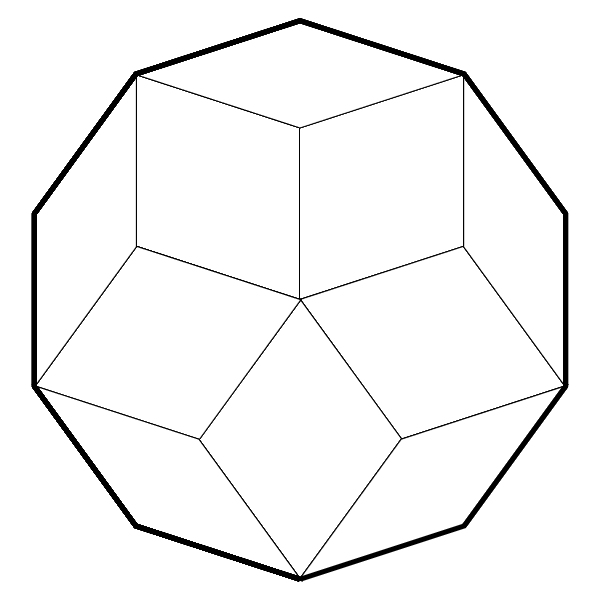
\includegraphics[width=5in]{imageserver/uploadimages/image7.png}
	\caption{Penrose.}
\end{figure}

\begin{figure}
	\centering
	
\includegraphics[width=5in]{imageserver/uploadimages/image18.png}
	\caption{Golden Spiral.}
\end{figure}

\begin{figure}
	\centering
	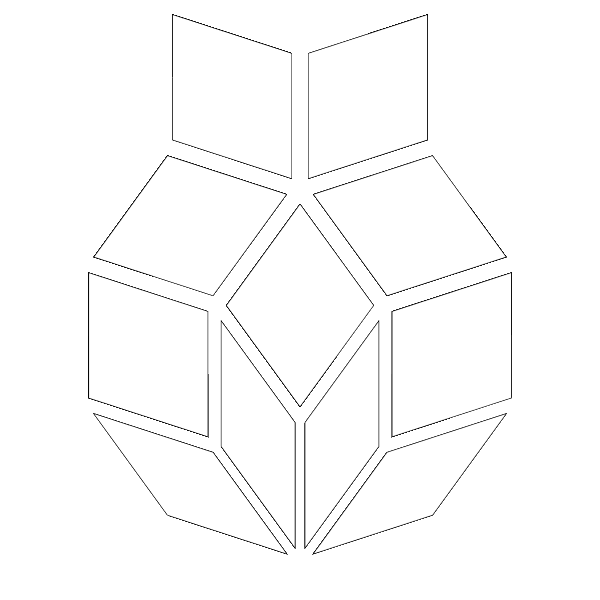
\includegraphics[width=5in]{imageserver/uploadimages/image8.png}
	\caption{Raspberry pi pattern for stitching felt onto bags.}
\end{figure}

\begin{figure}
	\centering
	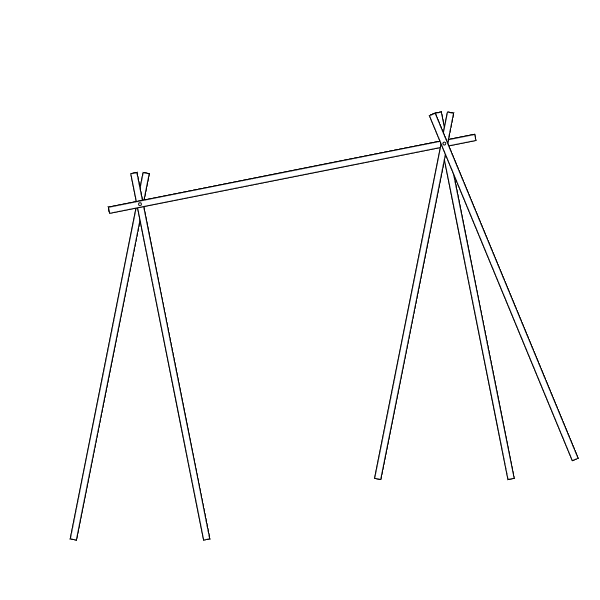
\includegraphics[width=5in]{imageserver/uploadimages/image9.png}
	\caption{Skeletron.}
\end{figure}

\begin{figure}
	\centering
	
\includegraphics[width=5in]{imageserver/uploadimages/image10.png}
	\caption{S Hook.}
\end{figure}

\begin{figure}
	\centering
	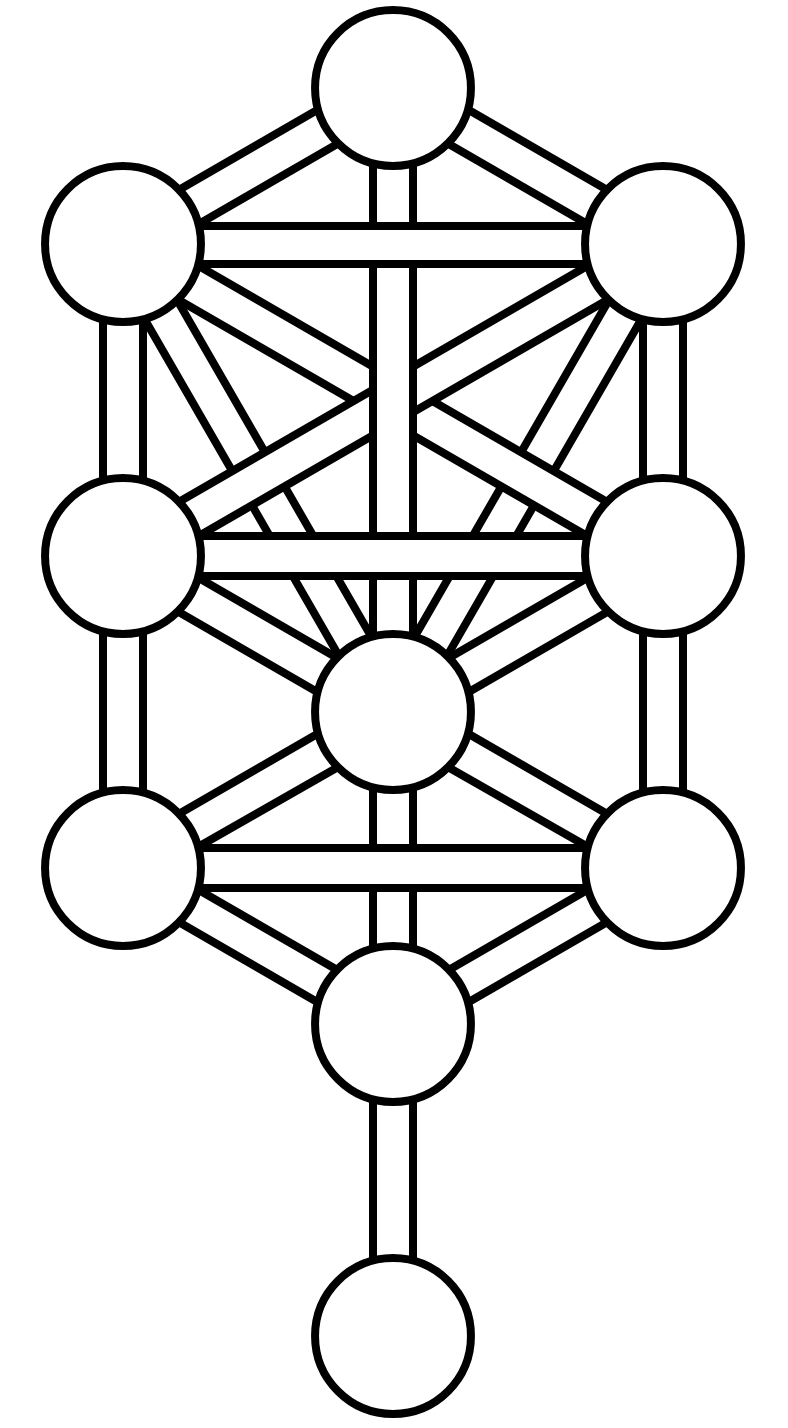
\includegraphics[width=3in]{imageserver/uploadimages/image1.png}
	\caption{Tree of life.}
\end{figure}




\end{document}